
\documentclass[journal]{IEEEtran}
\usepackage{cite}
\usepackage{amsmath,amssymb,amsfonts}
\usepackage{algorithmic}
\usepackage{graphicx}
\usepackage{textcomp}
\usepackage{xcolor}
\usepackage[all]{nowidow}
\usepackage[none]{hyphenat}

% \usepackage[switch  ]{lineno}

\def\BibTeX{{\rm B\kern-.05em{\sc i\kern-.025em b}\kern-.08em
T\kern-.1667em\lower.7ex\hbox{E}\kern-.125emX}}

\begin{document}

% \linenumbers

\title{Patrolling Robot with Facial Detection}

\author{
	\IEEEauthorblockN{
		Manisha Dhage\IEEEauthorrefmark{1}
		Vivek Ghuge\IEEEauthorrefmark{2},\\
		Divija Godse\IEEEauthorrefmark{3},
		Mitrajeet Golsangi\IEEEauthorrefmark{4},
		Pravin Harne\IEEEauthorrefmark{5},
	}
	\IEEEauthorblockA{
		\textit{dept. of Computer Science} \\
		\textit{Vishwakarma Institute of Technology}\\
		Pune, India\\
		Email : \IEEEauthorrefmark{1}manisha.dhage@vit.edu,
		\IEEEauthorrefmark{2}vivekghuge2002@gmail.com,
		\IEEEauthorrefmark{3}divijagodse@gmail.com,
		\IEEEauthorrefmark{4}mitrajeetgolsangi@gmail.com,
		\IEEEauthorrefmark{5}sunnyharne008@gmail.com,
	}
}

\maketitle

\begin{abstract}
	Security of any facility and the people inside it is a 	huge responsibility of the management of that facility. This, even though it can be achieved using humans, it leaves them at risk and introduces a factor of human
	error. Thus, The proposed system aims to improve the
	surveillance and security of a compound, without
	putting any human lives at risk and naturally removing
	the human error factor from the process. The paper
	discusses the implementation of such a system and all the
	work related to it. The proposed system is a fully
	functional robot which can follow the direction of a sound.
	It also has an on board camera which sends live footage
	of everything to a server. This feed is then processed
	for detection of a face and it is displayed to the user.
\end{abstract}

\begin{IEEEkeywords}
	security, IoT, facial detection, patrolling, arduino,
\end{IEEEkeywords}

\section{Introduction}
For billions of years mankind has faced threats which were potentially
life threatening and has found ingenious ways to overcome them. Even
so, one of the most pressing concerns in society today still remains
the safety of its citizens. The threats in today's modern day world
are not as simple as a lion attacking a human like the good old days,
but have developed as the civilization has evolved. Sadly the measures
to counteract these threats are not improving at the same speed.
As it is rightly said by John Maxwell “Change is inevitable, but
growth is optional”. According to a research conducted in
\cite{[17]} the acid attacks on women in south Asian
countries are still prevailing and cause a great deal of
damage to the women. It was not until 2019 that Bangladesh
could reduce the frequency of these attacks by a mere 20-30\%.
Another survey says that 38.7\% of youths which were interviewed
showed signs of committing at least one hate crime \cite{[18]}.

All the above is evidence that even in the 21st century the crimes
are at an all time high and don't seem to be going down.
Even though we have various measures to prevent or stop such
threats all of them involve human lives being put in danger.
This system has been put as a last resort and not as a
foolproof solution. The bypass to this system has become
so common that even in crime thrillers it is a common
practice to introduce at least one scene in which the convict
can slip through the “secure” facility when the guards are
changing shifts.

Thus, in order to reduce the risk of any further human being
and remove the possibility of any human error the idea of
the proposed system was put forth by the team. As this is a
well researched field the team found lots of research papers
which helped improve the overall concept and make the world a
little safer.

\section{Literature Review}
One of the most important needs of modern times is
security. The rise in population is directly proportional
to the need for proper security. A night patrolling
visionary robot would help achieve certainty, especially
during the night. All the research papers have directed
to the fact that the basic must-haves for the night
patrolling systems are the logic for sound sensing,
moving towards the area of target and back to the
original location, image capturing and processing.

The night vision patrolling robot has the primary
objective to ensure the safety of the people without
putting any human life at risk. There are certain
essential features needed in the robot, such as a night
vision, obstacle detection, and motor driver circuits
for controlling them\cite{[1]}. All of these are controlled
using a microcontroller board such as an Arduino UNO
or raspberry pi. In addition, a wireless IR transceiver
would be helpful in the navigation of the robot\cite{[3]}.
According to \cite{[1]} the proposed system has the best
advantage over disadvantage ratio if it uses an IR
Camera with a wireless controller and some form of
an obstacle detection system. Furthermore, optional
features such as a GPS Module, GSM radios \cite{[3]}, sound
sensor\cite{[1]} will greatly help increase the productivity
of the project.
Journals have shown that a sound sensor and a smart
camera are primary necessities for the system. Along
with this according to the paper by N.Hemavathi the
robot is built with a DC motor and transistors.
The movement of the robot is handled by multiple
logics operated on the transistors. These transistors
allow the motion of the DC motor in the desired
direction\cite{[6]}. Bluetooth technology has also been
used in the process for serial communication with
the robot\cite{[7]}. In another paper, the authors have
mentioned the use of a special GPS for location tracking.
Object detection algorithms have been designed for the
robot to understand the route\cite{[8]}.
Technology is advancing at a rapid pace nowadays. These
shifts are also visible in the robotics industry. As a
result, the system suggested in the given papers reflects
the current state of the field. The main objective of this
is to offer ladies safety at night. Using a credit-card-sized
Raspberry Pi and an open CV, the author of this paper,
created a night patrolling robot (computer vision).\cite{[11]}
To detect the face, the suggested system employs a Raspberry
Pi camera. Anomaly detection is done using deep learning
technologies\cite{[13]}. As a result, the image is recorded using
the pi camera and sent to the raspberry pi for face and
human detection using OpenCV.  The accuracy of this
approach is around 83 percent\cite{[11]}.The sensors used are
IR sensors and sound sensors. According to this project,
the entire territory monitoring is completed using a night
vision camera and a programmed framework. When a sound is
detected, the robot will follow a certain path to that
space, capture the region, and send the picture to the
user via IoT. Behind this project is a pre-programmed
dazzling path for night vision viewing.\cite{[12]}
The proposed system focuses on the security of the place
where it is implemented. It is specially designed to
carry out the security assessment function at the night
time when it will be dark all over the place. It is equipped
with a night vision camera which will be used to capture
the pictures of the spot if any suspicious activity takes
place. It moves on a predestined path, and it moves in
the direction of sound. It is also equipped with human
face recognition technology. This system uses the LAN
protocol of IOT, and it sends the recorded images to the
responsible authority so that they can take any actions
if necessary. It system uses a microcontroller, night
vision cameras, sound sensors, Infrared sensor and Motor
drivers.\cite{[15]}
This system is built to ensure women safety in remote
regions and public places. IOT gecko is used for
receiving transmitted snapshots and displaying them to
people with alert sounds. This system consists of a
combination of 2 HD cameras to monitor the environment
sharply and closely. The hardware used in this system are
HD infrared camera with night vision, Sound sensor,
DC motor, IR Sensor, Ultrasonic sensor, LCD display, and
a motor driver.\cite{[16]}

Facial recognition is an important aspect in terms of the
proposed system. This serves a greater importance in order
to assess the threat and act accordingly.\cite{[2]} Facial
recognition is a subset of the highly expanding computer
vision field. This field has been overly dominated by the
areas of Machine Learning and Deep Learning from the very
beginning\cite{[5]}. Taking into consideration the scope of
lighting in a night patrolling robot it is safe to assume
that the best approach would be to perform IR recognition\cite{[2]}.
Thus according to \cite{[2]} the best possible way of training
the TIR based facial recognition is to use a Deep CNN
Classifier with substantial training data. The losses
given by equation 1
\begin{equation}
	\sum_i^N[\| \int (x_i^a) - \int (x_i^p)\|_2^2 - \| \int (x_i^a) - \int (x_i^n)\|_2^2 + \alpha]
\end{equation}
Are the minimum and give the best possible output with a
method called triple loss learning.\cite{[2]} There are
three main steps for facial recognition and tracking in
real time\cite{[4]}. The First Step is Detection of Faces to track
them, the next being recognition of facial features, which is determined
using equation 2
\begin{equation}
	\begin{aligned}
		\Omega^m_{[w, h]} =
		 & \begin{pmatrix}
			   [\frac{m}{w}] + [\frac{m - 1}{w}] + \ldots + [\frac{w + 1}{w}] + 1
		   \end{pmatrix}
		\cdot                                                                          \\
		 & \begin{pmatrix}
			   [\frac{m}{h}] + [\frac{m - 1}{h}] + \ldots + [\frac{h + 1}{h} + 1]
		   \end{pmatrix}
	\end{aligned}
\end{equation}
The last step is to begin tracking the face in real time.

Object detection bases the image processing. The image is
seen in a digital form of the same. Process of Image
processing, object detection majorly involves object recognition,
object localisation, image classification. According to a
survey for different processes for image processing,
multiple techniques have been identified which present
different accuracies for the same. The survey paper implies
that numerous techniques have separate sets of specifications.
For example, Deep CNN shows 85\% sensitivity especially for
medical cases, face recognition vendor test (FRVT) makes
identifying a male easier than female. According to this paper,
Deep neural networks and CNN which are AI based techniques are
recommended for object detection \cite{[9]}.  Furthermore, another
paper by Sandeep Kumar, has emphasized on the kind of image
processed. It mentions the use of Convoluted neural networks,
for static images with static background. After preprocessing,
and feature extraction, single neural networks are integrated
for image recognition and processing\cite{[10]}.

The author of this work presents several innovative models for
all stages of a face recognition system. To perform the process
of face detection efficiently, the authors suggest a hybrid
model integrating AdaBoost and Artificial Neural Network (ABANN).
The labeled faces detected by ABANN will then be aligned using
the Active Shape Model and Multi-Layer Perception in the next
stage. The author proposes a novel 2D local texture model based
on Multi-Layer Perceptron in this alignment step. The model's
classifier enhances the accuracy and robustness of local
searching on faces with ambiguous outlines and expression
variation. The authors of the research offer a way for boosting
efficiency in the feature extraction step by combining two
methods: geometric feature-based method and Independent
Component Analysis method.\cite{[14]}

\section{Related Work}
\subsection{Haar Cascade Classifier}
One of the most popular study topics is the facial detection
system. This section discusses the work defined by prior
scholars on facial detection. Face detection algorithms and
approaches have been the subject of numerous investigations.

For the algorithm, Harleen Kaur and Arisha Mirza used OpenCV
and NumPy, and they divided facial recognition into two parts.
The first step in this technique is the classification task,
which takes any random image or media as input and outputs a
binary value of yes or no, indicating whether or not there are
any faces in the image. The second phase is a face localization
job, which takes an image as input and outputs the location of
any face within that picture in a bounding box with width and
height parameters.\cite{kaur2021face}

Di Lu and Limin Yan describe that In the field of face detection,
the OpenCV approach is widely used. It begins by extracting the
face from a big sample set and then extracting the feature
photos. The face detector is Haar characteristics in the image,
followed by the AdaBoost algorithm. The algorithm detects
faces. can easily adapt to challenging conditions, such as
insufficient illumination and backdrop blur, resulting in a
significant improvement in performance.\cite{lu2021face}

The author of the last paper describes various algorithms which
are available for face detection. The author of this paper says
that their paper is for anyone interested in learning about
the various types of face detection algorithms. The following
is how the rest of the paper is structured: first, they go
over the feature-based techniques in more detail. After that
the image-based techniques are discussed. Also., the face
detection techniques are compared in a thorough manner.\cite{hasan2021human}

The Haar Cascade technique is an Object Detection Algorithm
that may be used to recognize faces in images or real-time
videos. Viola and Jones proposed edge or line detection
features in their research paper.\cite{viola2001rapid}
Features are one of the most significant aspects of the haar
cascade approach. This trait is depicted in Fig. \ref{haar_features}.
These elements on the image make it simple to locate the image's
boundaries or lines, as well as locations where the brightness
of the pixels abruptly shift.

\begin{figure}[!ht]
	\centering
	
\includegraphics[width=\linewidth]{./img/HaarCascadeWorking.jpeg.png}
	\caption{A sample of Haar feature \cite{viola2001rapid}}
	\label{haar_features}
\end{figure}

Pixels with a value of 1 are darker in the haar feature,
while pixels with a value of 0 are lighter. Each of these
is in charge of identifying a specific feature in the image.
Any structure in the image where there is a quick change of
intensities, such as an edge, a line, or any other structure.
The goal is to calculate the sum of all image pixels in the
darker part of the haar feature, as well as the sum of all
image pixels in the lighter portion of the haar feature.
Then figure out how they differ. The haar value will be
closer to 1 if the image has an edge dividing dark pixels
on the right from light pixels on the left. That is, if the
haar value is closer to 1, we claim there is an edge detected.
There is no edge in the example above because the haar value
is distant from 1. The haar feature must traverse the entire
image to detect an edge anyplace in it.

\subsection{MediaPipe by Google}
Another popular framework for facial detection is MediaPipe
developed by Google. It has many features like object
detection, facial detection, posture recognition, facial
recognition and more. Fig. \ref{internalWorkings} shows the internal workings
of the mediapipe framework \cite{mediapipe}

\begin{figure}[!ht]
	\centering
	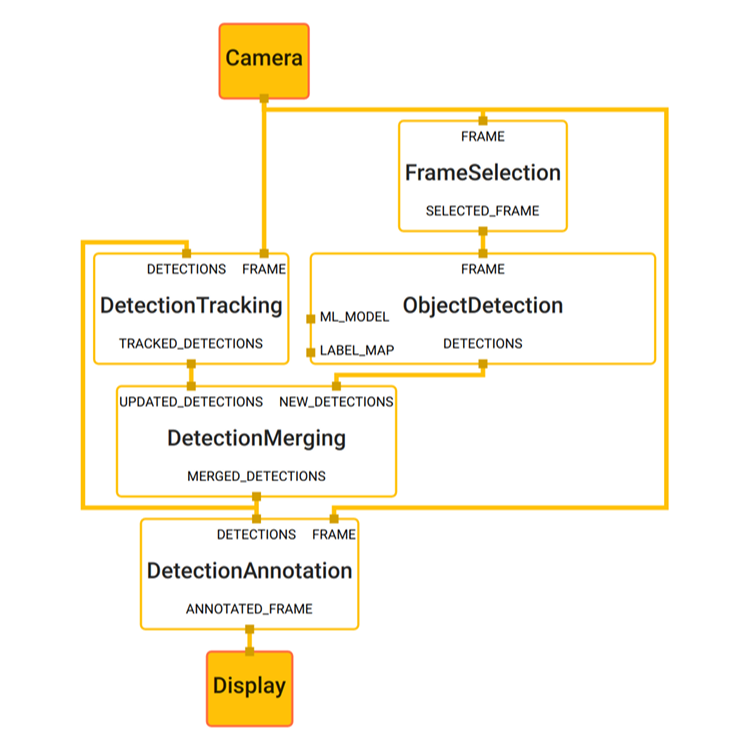
\includegraphics[width=\linewidth]{./img/MediaPipeImplementation.png}
	\caption{Media Pipe Internal Workings}
	\label{internalWorkings}
\end{figure}
MediaPipe uses a unique architecture which allows the user to
incrementally prototype a pipeline. Here each component is a
calculator. Graphs are specified in the Graph object using the
GraphConfig Protocol. Data streams connect the Graphs and
Calculators where each stream is a time-series of data packets \cite{mediapipe}

\section{Methodology}
\subsection{Hardware}
\subsubsection{Arduino UNO}
Arduino UNO is a microcontroller board based on ATmega328p.
The board has a set of input and output digital pins as
well as analog pins. The board can be interfaced with
several other expansion boards. The Arduino board presents
a facility for communicating with computers.
\subsubsection{DC motors}
DC motors belong to a class of rotatory motors, which convert
DC current into Mechanical energy. Using this principle, the
DC motors would act as an agency for mobility.
\subsubsection{Gyroscope (GY521)}
This is a breakout board which consists of a 3 axis gyroscope,
3 axis accelerometer, and a temperature sensor. Gyroscope
helps in calculating the orientation and the angular velocity.
The digital motion processor can be used to process complex
algorithms on board.
\subsubsection{Ultrasonic sensors}
Ultrasonic sensors are used to measure the distance of any
object in the vicinity of the sensor. It has a wide range
and uses the emission and detection of ultrasonic waves as
the principle. Primarily ultrasound sensors are used for
the purpose of object detection in the proposed system.
\subsubsection{ArduCam mini}
ArduCam mini is a high definition 2MP SPI camera, which
reduces the complexity of camera control interfaces.
It integrates 2MP CMOS image sensor OV2640, and provides
miniature size, as well as the easy to use hardware
interface and open source code library.

\subsection{Software}
The software part of the proposed methodology is further subdivided
into 2 parts the first being the Flutter application and the second
being the facial detection. The Flutter application serves as a
Frontend / User Interface for the system, it notifies the user
about the status of the robot using the live feed of the onboard
camera from the actual robot. The workflow of this application
is explained in Fig. \ref{workflow}
\begin{figure}[!ht]
	\centering
	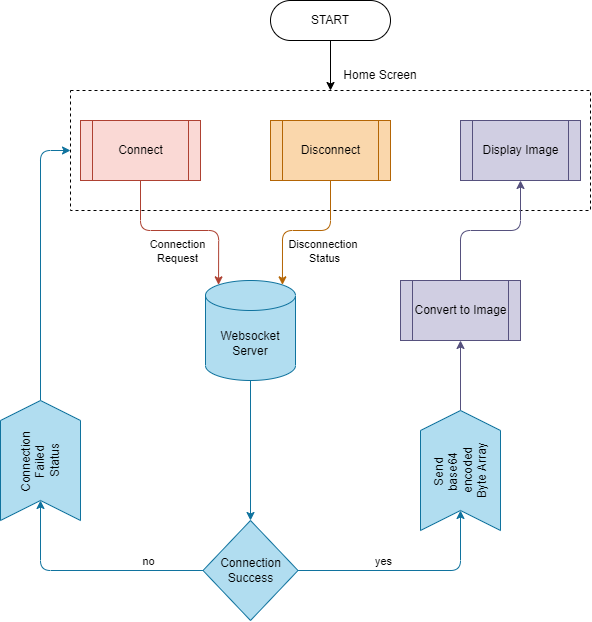
\includegraphics[width=\linewidth]{./img/flutter_implementation.png}
	\caption{Application workflow}
	\label{workflow}
\end{figure}
Now in Fig. \ref{workflow} as you can see the Flutter application
only makes a connection request to the websocket. This is because
as mentioned earlier the websocket protocol can directly dump
data on the client without it specifically requesting for any data.
The websocket server serves a simple purpose in this application.
It first reads the data from the camera (which is the live video
feed), frame by frame and then it performs facial detection tasks
on that frame. The program then writes the confidence percentage
on the image and then reads it as a byte array. This byte array
is encoded in a base64 string and packaged and sent from the
server to the client side. The Flutter client then reads this
string and decodes it which in turn leaves it with a byte array,
it then renders that byte array onto the application thus giving
the user a face detected live video feed.

\begin{figure}[!ht]
	\centering
	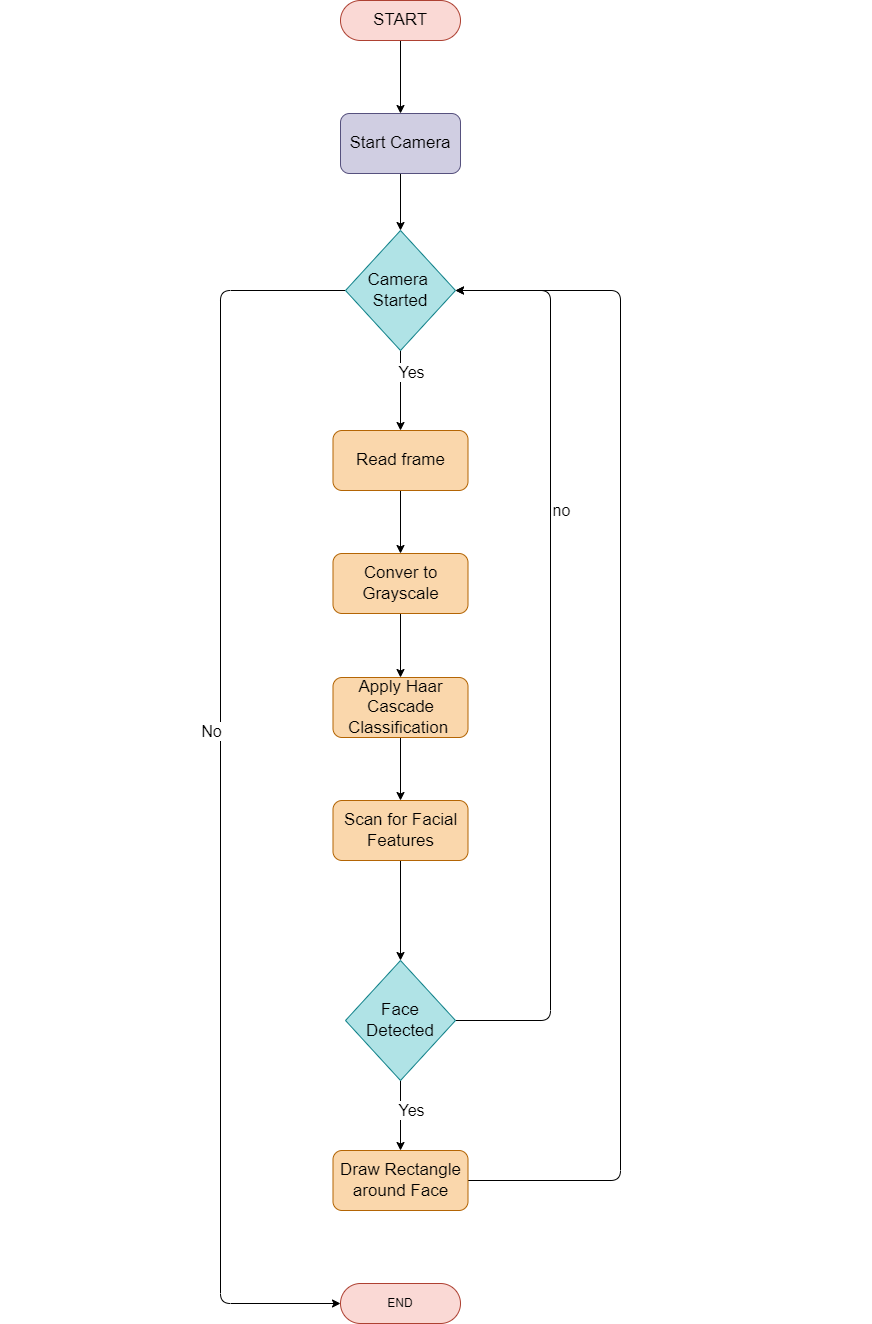
\includegraphics[width=\linewidth]{./img/HaarFlowchart.dio.png}
	\caption{Flowchart for implemented model}
	\label{haar_flowchart}
\end{figure}

As illustrated in Fig. \ref{haar_flowchart}, the camera should
be started first; if there is a problem with the camera opening,
the code will be terminated. Then it will read the frame/image
identified by the camera; Haar cascade is a grayscale
image-only algorithm, hence the acquired image must first be
transformed to grayscale before the algorithm can be applied.
The frame is now ready for the haar cascade algorithm to run.
The algorithm will scan the facial feature after passing
through the haar cascade classifier to determine the face in
that frame or image. If a face is detected, a rectangle will
be drawn around it. Otherwise, the code will be terminated.

% \section{Results and Discussion}

% \section{Conclusion}

% \pagebreak

\bibliographystyle{IEEEtran}
\bibliography{references.bib}

\end{document}
